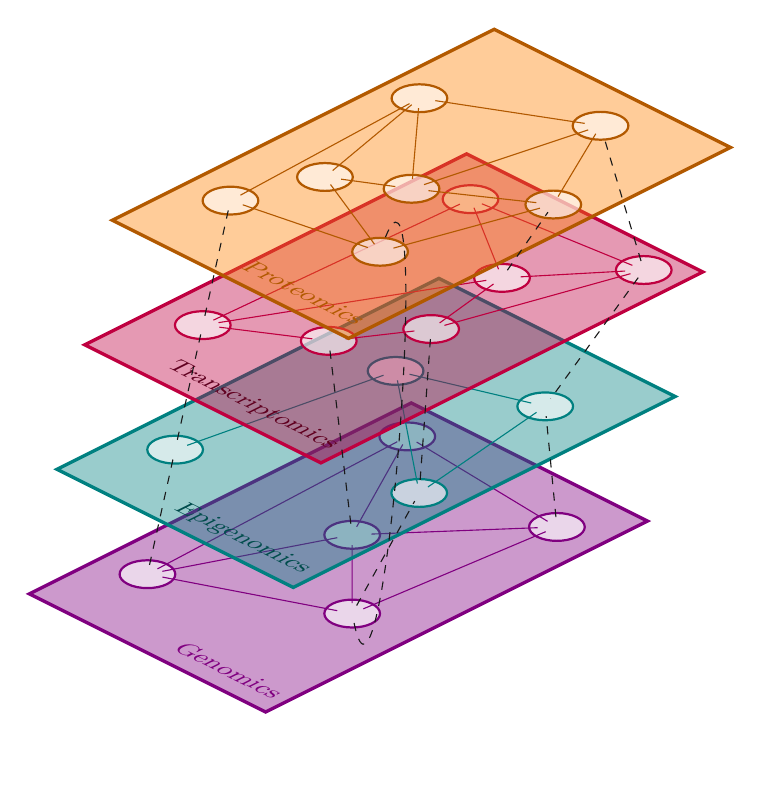
\begin{tikzpicture}
    \begin{scope}[
            yshift=0,
            yslant=-0.5,xslant=1,
            every node/.append style={yslant=-0.5,xslant=1}
        ]
        \fill[violet,fill opacity=0.4] (0,0) rectangle (3,4.85);
        \draw[violet,very thick] (0,0) rectangle (3,4.85);
        \draw[violet, thick, fill=white, fill opacity=0.6] (0.5,1) circle (2.5mm) node (G1) {};
        \draw[violet, thick, fill=white, fill opacity=0.6] (2.3,1.8) circle (2.5mm) node (G2) {};
        \draw[violet, thick, fill=white, fill opacity=0.6] (1.3,2.8) circle (2.5mm) node (G3) {};
        \draw[violet, thick, fill=white, fill opacity=0.6] (2.5,4.2) circle (2.5mm) node (G4) {};
        \draw[violet, thick, fill=white, fill opacity=0.6] (0.4,4.4) circle (2.5mm) node (G5) {};

        \node[anchor=east, font=\footnotesize, text=violet] at (3,0.3) {Genomics};
        \draw[violet] (G1) -- (G2);
        \draw[violet] (G1) -- (G3);
        \draw[violet] (G4) -- (G3);
        \draw[violet] (G2) -- (G4);
        \draw[violet] (G2) -- (G3);
        \draw[violet] (G3) -- (G5);
        \draw[violet] (G4) -- (G5);
        \draw[violet] (G1) -- (G5);
    \end{scope}

    \begin{scope}[
            yslant=-0.5,xslant=1,
            every node/.append style={yslant=-0.5,xslant=1},
            yshift=50, xshift=-40
        ]
        \fill[teal,fill opacity=0.4] (0,0) rectangle (3,4.85);
        \draw[teal,very thick] (0,0) rectangle (3,4.85);
        \draw[teal, thick, fill=white, fill opacity=0.6] (0.5,1) circle (2.5mm) node (E1) {};
        \draw[teal, thick, fill=white, fill opacity=0.6] (0.9,3.4) circle (2.5mm) node (E2) {};
        \draw[teal, thick, fill=white, fill opacity=0.6] (2.6,2) circle (2.5mm) node (E3) {};
        \draw[teal, thick, fill=white, fill opacity=0.6] (2.3,3.9) circle (2.5mm) node (E4) {};
        \node[anchor=east, font=\footnotesize, text=teal!60!black] at (3,0.3) {Epigenomics};

        \draw[teal] (E1) -- (E2);
        \draw[teal] (E4) -- (E2);
        \draw[teal] (E4) -- (E3);
        \draw[teal] (E2) -- (E3);

        \draw[black!90, dashed] (G1) -- (E1);
        \draw[black!90, dashed] (G4) -- (E4);
        \draw[black!90, dashed] (G2) -- (E3);
        %\draw[black!90, dashed] (G3) -- (E2);
    \end{scope}

    \begin{scope}[
            yslant=-0.5,xslant=1,
            every node/.append style={yslant=-0.5,xslant=1},
            yshift=100, xshift=-80
        ]
        \fill[purple,fill opacity=0.4] (0,0) rectangle (3,4.85);
        \draw[purple,very thick] (0,0) rectangle (3,4.85);
        \draw[purple, thick, fill=white, fill opacity=0.6] (0.5,1) circle (2.5mm) node (T1) {};
        \draw[purple, thick, fill=white, fill opacity=0.6] (0.6,4.3) circle (2.5mm) node (T2) {};
        \draw[purple, thick, fill=white, fill opacity=0.6] (2.6,4.5) circle (2.5mm) node (T3) {};
        \draw[purple, thick, fill=white, fill opacity=0.6] (2,2.4) circle (2.5mm) node (T4) {};
        \draw[purple, thick, fill=white, fill opacity=0.6] (1.5,1.6) circle (2.5mm) node (T5) {};
        \draw[purple, thick, fill=white, fill opacity=0.6] (1.8,3.5) circle (2.5mm) node (T6) {};
        \node[anchor=east, font=\footnotesize, text=purple!50!black] at (3,0.3) {Transcriptomics};

        \draw[purple] (T1) -- (T2);
        \draw[purple] (T1) -- (T5);
        \draw[purple] (T4) -- (T5);
        \draw[purple] (T4) -- (T6);
        \draw[purple] (T4) -- (T3);
        \draw[purple] (T3) -- (T6);
        \draw[purple] (T2) -- (T6);
        \draw[purple] (T2) -- (T3);
        \draw[purple] (T1) -- (T6);

        \draw[black!90, dashed] (T1) -- (E1);
        \draw[black!90, dashed] (T3) -- (E4);
        \draw[black!90, dashed] (T4) -- (E3);
        \draw[black!90, dashed] (T5) -- (G3);
    \end{scope}

    \begin{scope}[
            yslant=-0.5,xslant=1,
            every node/.append style={yslant=-0.5,xslant=1},
            yshift=150, xshift=-120
        ]
        \fill[orange,fill opacity=0.4] (0,0) rectangle (3,4.85);
        \draw[orange!70!black,very thick] (0,0) rectangle (3,4.85);
        \draw[orange!70!black, thick, fill=white, fill opacity=0.6] (0.5,1) circle (2.5mm) node (P1) {};
        \draw[orange!70!black, thick, fill=white, fill opacity=0.6] (0.8,1.9) circle (2.5mm) node (P2) {};
        \draw[orange!70!black, thick, fill=white, fill opacity=0.6] (0.4,3.5) circle (2.5mm) node (P3) {};
        \draw[orange!70!black, thick, fill=white, fill opacity=0.6] (2.6,3) circle (2.5mm) node (P4) {};
        \draw[orange!70!black, thick, fill=white, fill opacity=0.6] (1.9,4.3) circle (2.5mm) node (P5) {};
        \draw[orange!70!black, thick, fill=white, fill opacity=0.6] (1.5,2.3) circle (2.5mm) node (P6) {};
        \draw[orange!70!black, thick, fill=white, fill opacity=0.6] (2.1,1.3) circle (2.5mm) node (P7) {};

        \node[anchor=east, font=\footnotesize, text=orange!70!black] at (3,0.3) {Proteomics};
        \draw[orange!70!black] (P1) -- (P3);
        \draw[orange!70!black] (P3) -- (P5);
        \draw[orange!70!black] (P3) -- (P6);
        \draw[orange!70!black] (P6) -- (P5);
        \draw[orange!70!black] (P2) -- (P7);
        \draw[orange!70!black] (P4) -- (P5);
        \draw[orange!70!black] (P4) -- (P7);
        \draw[orange!70!black] (P1) -- (P7);
        \draw[orange!70!black] (P6) -- (P4);
        \draw[orange!70!black] (P6) -- (P2);
        \draw[orange!70!black] (P3) -- (P2);

        \draw[black!90, dashed] (T1) -- (P1);
        \draw[black!90, dashed] (T3) -- (P5);
        \draw[black!90, dashed] (T6) -- (P4);
        \draw[black!90, dashed] (G2) to [bend right=172] (P7);

    \end{scope}

\end{tikzpicture}